\documentclass[11pt,a4paper]{article}
\usepackage[utf8]{inputenc}
\usepackage{amsmath}
\usepackage{amsfonts}
\usepackage{amssymb}
\usepackage{enumerate}
\usepackage{graphicx}
\usepackage{enumitem}



\title{Lab 01\\Arquitectura de Computadores \\ Sección 2}
\author{Joaquín Ramírez}
\begin{document}
\maketitle
\begin{enumerate}
\item Dados dos números de 4-bits, se comparan los pares i-ésimos, $i = 0, 1, 2, 3$ con XOR gates. Finalmente se conectan en un AND gate, el cual solo se activará cuando todos los pares estén activados.
\begin{figure}[h!]
\centering
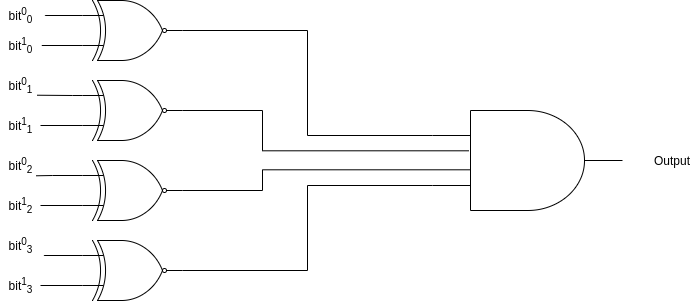
\includegraphics[scale=0.4]{1.png} 
\end{figure}
\\
Si solo se pueden utilizar 2-input XNOR y 2-input AND gates, entonces el diagrama cambia.
\begin{figure}[h!]
\centering
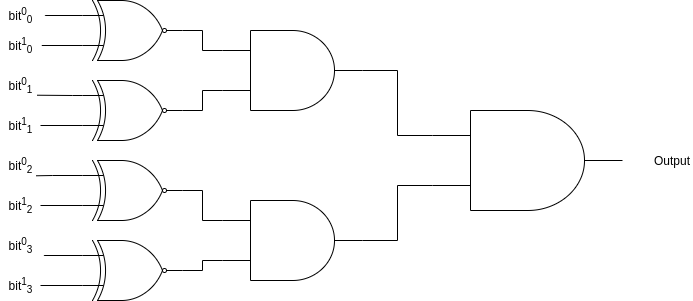
\includegraphics[scale=0.4]{0.png} 
\end{figure}
\item Se adjunta la simulación en LTSpice del ejercicio anterior.
\\
\\
\begin{figure}[h!]
\centering
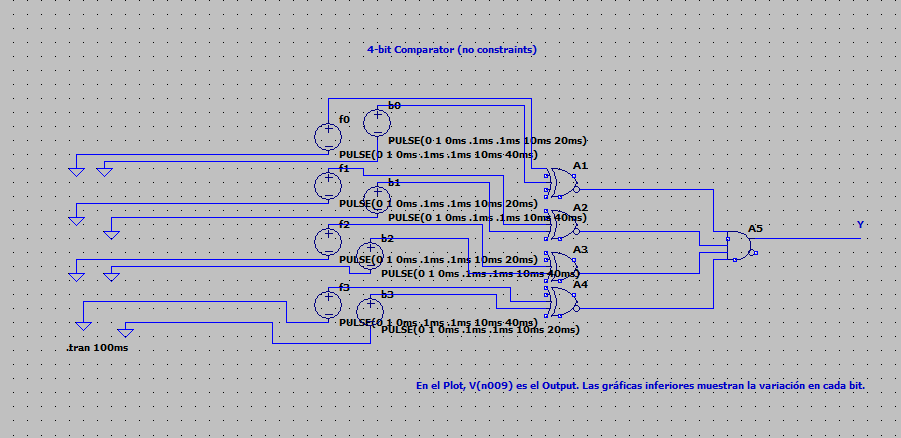
\includegraphics[scale=0.4]{dia11.png} 
\end{figure}
\\
\begin{figure}[h!]
\centering
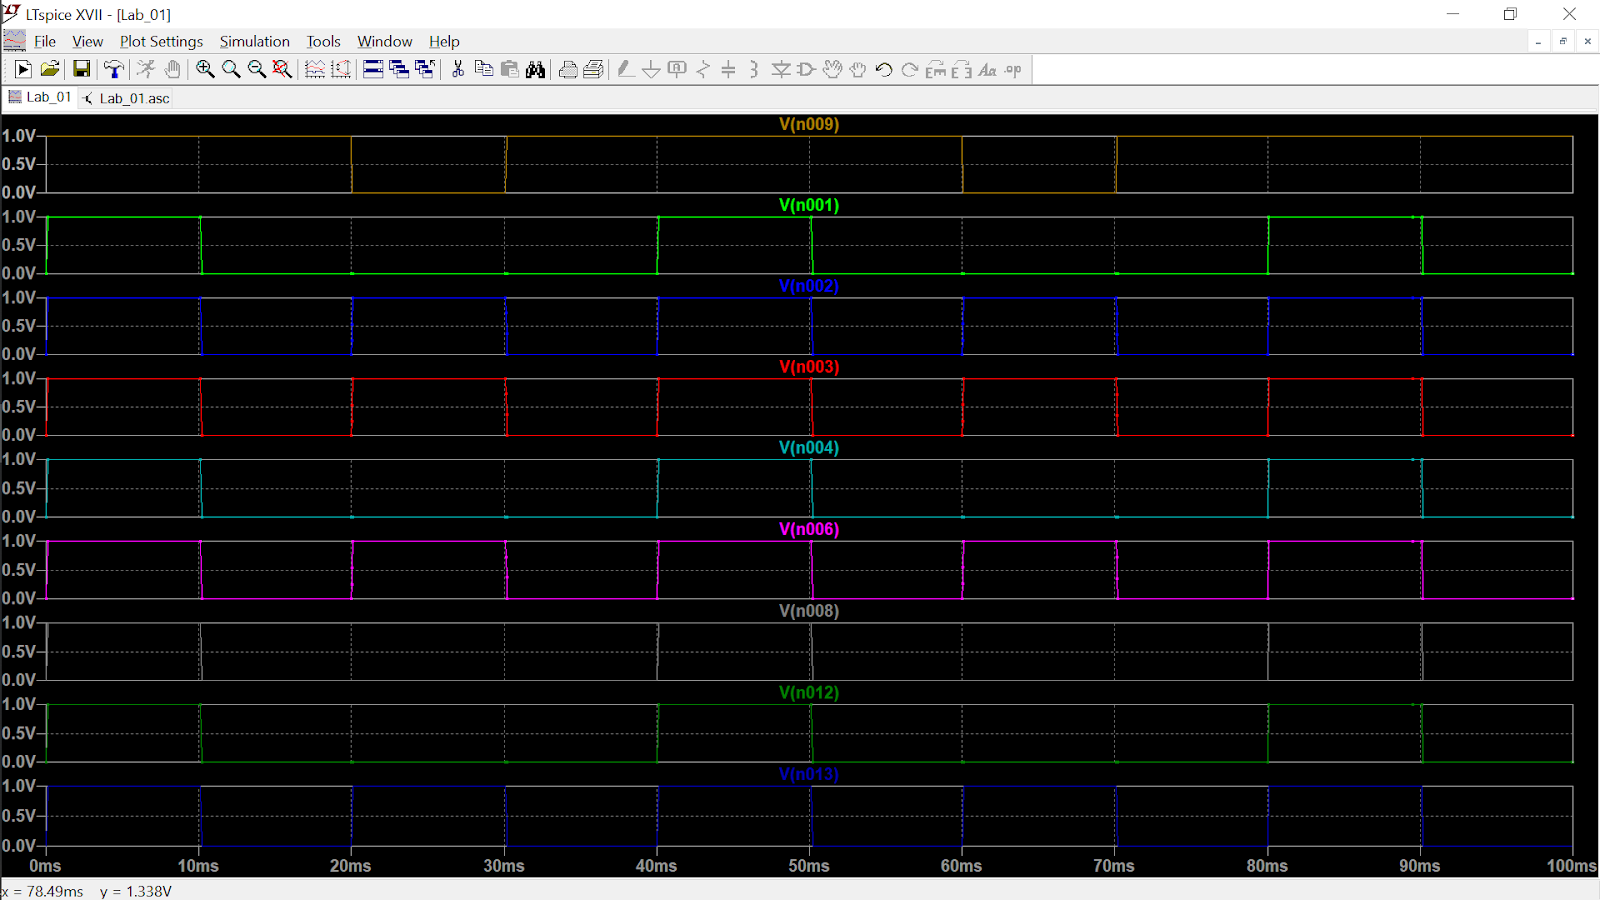
\includegraphics[scale=0.2]{plot11.png} 
\end{figure}
\\
\begin{figure}[h!]
\centering
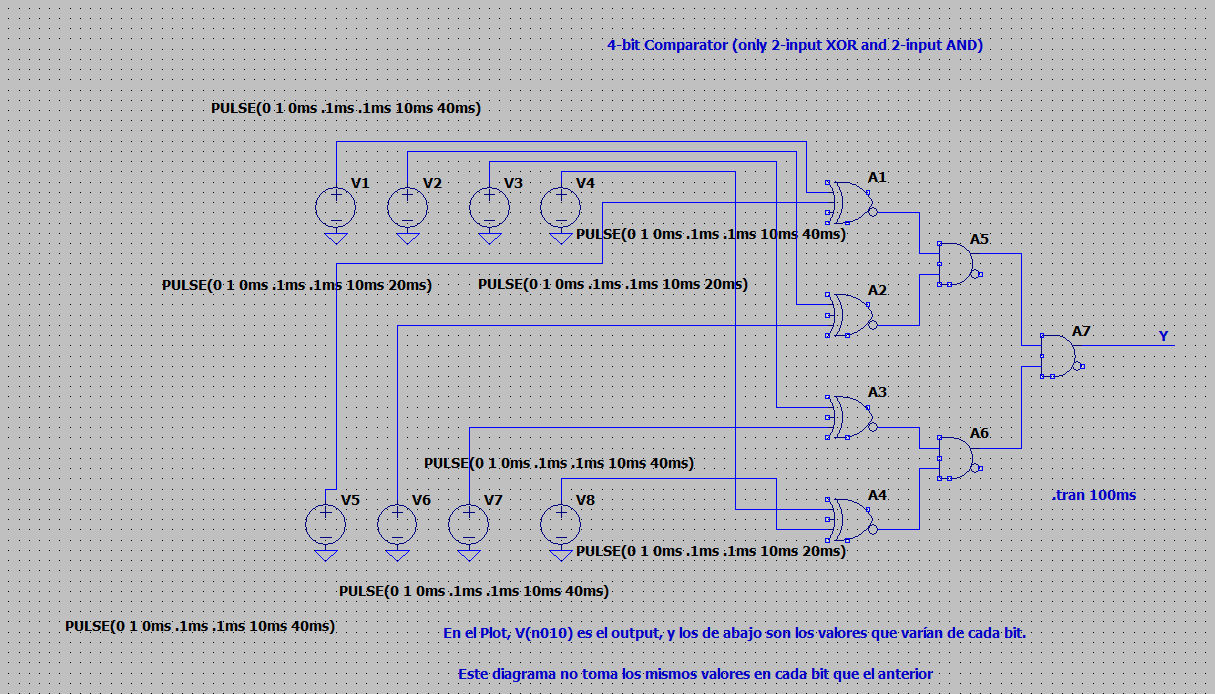
\includegraphics[scale=0.24]{dia12.png} 
\end{figure}
\begin{figure}[h!]
\centering
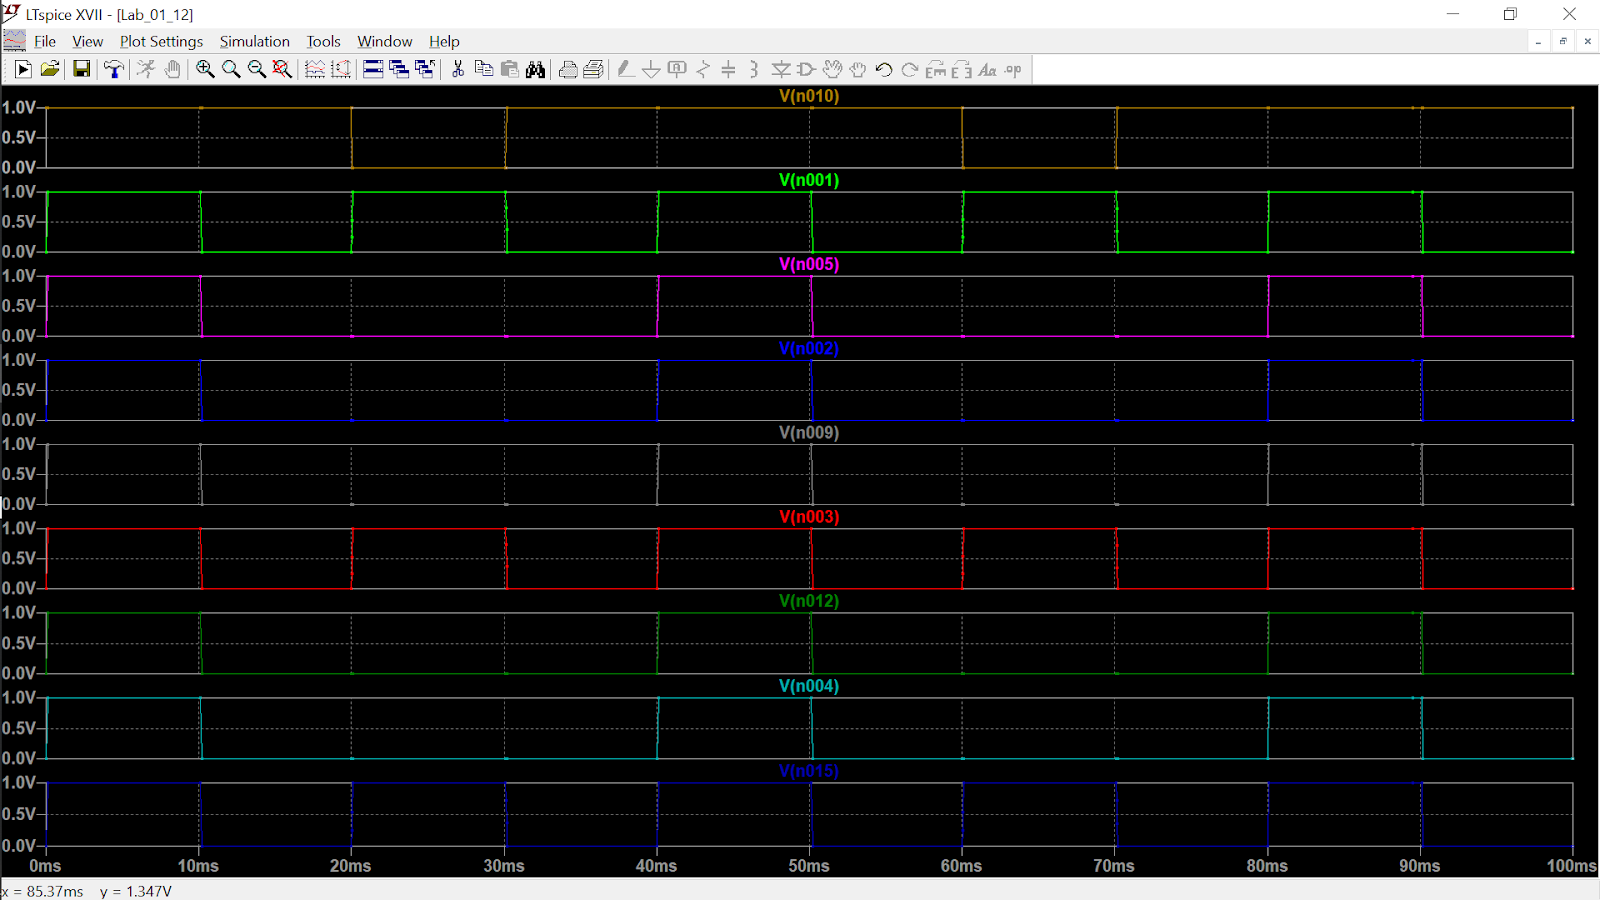
\includegraphics[scale=0.2]{plot12.png} 
\end{figure}

\item Los diagramas con NAND gates de ciertas funciones booleanas son:
\begin{itemize}
\item NOT: se divide un input en dos y pasa por un NAND, lo que significa que simplemente se invertirán los posibles casos 0 y 1.
\begin{figure}[h!]
\centering
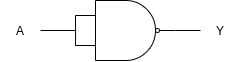
\includegraphics[scale=0.5]{2.png} 
\end{figure}
\item AND: se niega un NAND con el NOT del ejercicio anterior.
\begin{figure}[h!]
\centering
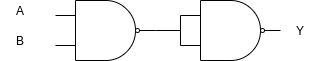
\includegraphics[scale=0.5]{3.png} 
\end{figure}
\\
\item XOR: Partiendo de la Suma de Productos podemos llegar a la forma simplificada del diagrama con NANDs.
 $Y = A\overline{B}+\overline{A}B=
 A\overline{B} + \overline{A}A + \overline{A}B + \overline{B}B=A(\overline{A}+\overline{B}) + B(\overline{A}+\overline{B}) = \overline{\overline{A(\overline{AB})}}+\overline{\overline{B(\overline{AB})}} = \overline{\overline{A(\overline{AB})} \    
 \overline{B(\overline{AB})}}$
 
\begin{figure}[h!]
\centering
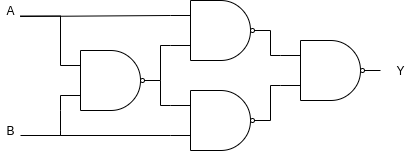
\includegraphics[scale=0.5]{6.png} 
\end{figure}
\pagebreak
\item XNOR: se aplica un NAND a la respuesta del XOR.
\\
\begin{figure}[h!]
\centering
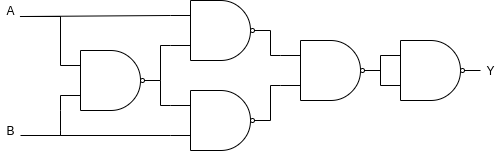
\includegraphics[scale=0.5]{7.png} 
\end{figure}
\\
A partir de esto, el comparador del inciso 1 quedaría de la \\ siguiente forma:
\begin{figure}[h]
\centering
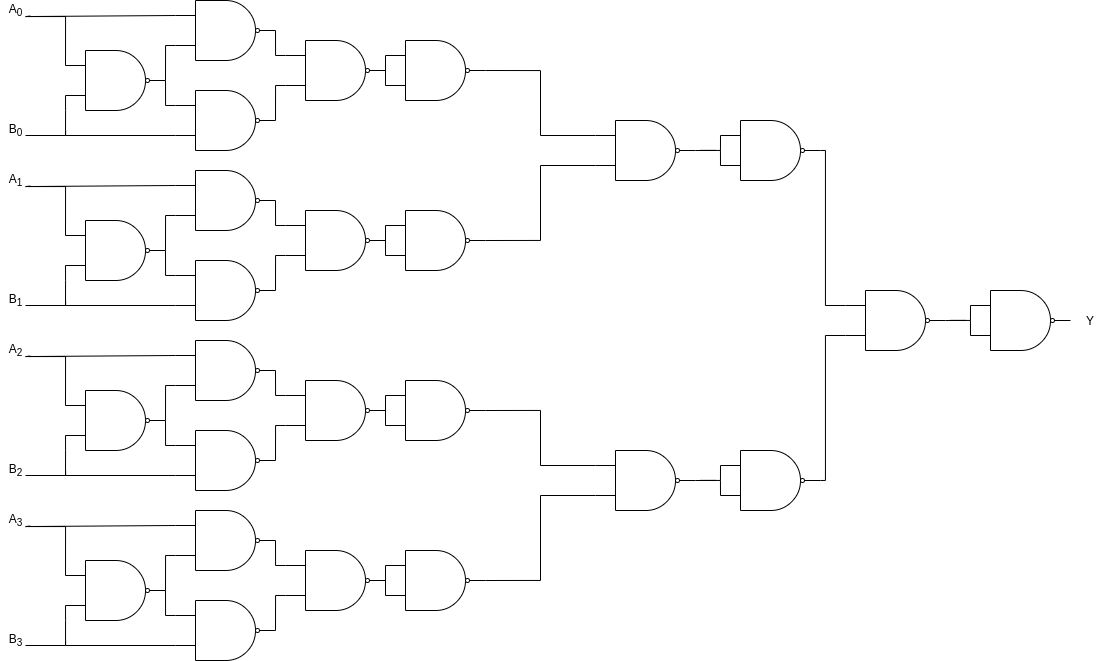
\includegraphics[scale=0.35]{comparator.png} 
\end{figure}
\end{itemize}
\item 
\begin{enumerate}[label=(\alph*)]

\item Siguiendo la lógica del ejercicio 1 y si no hay restricciones, se observa que la cantidad de compuertas XNOR es igual a $n$, donde n es el ńumero de bits. Después, se añade una compuerta AND, la que verifica si en efecto  todos los pares de bits son idénticos. Así, se puede decir que
$$\# \ compuertas = n + 1$$
Por otra parte, si solo se permiten compuertas de tipo 2-input, entonces
$$\# \ compuertas = n_{_{XOR}} + (n - 1)_{_{AND}}$$
\\
\begin{table}[h]
\centering
\begin{tabular}{|l|l|l|l|}
\hline
bits & XNOR gate & AND gate&Total\\
\hline
8&8&1&9\\
\hline
16&16&1&17\\
\hline
32&32&1&33\\
\hline
64&64&1&65\\
\hline
\end{tabular}
\end{table}
\\
\item Los comparadores en bloque son:
\begin{figure}[h]
\centering
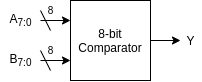
\includegraphics[scale=1]{8bit.png} 
\end{figure}
\begin{figure}[h]
\centering
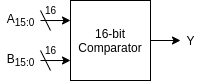
\includegraphics[scale=1]{16bit.png} 
\end{figure}
\begin{figure}[h!]
\centering
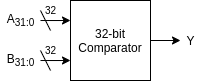
\includegraphics[scale=1]{32bit.png} 
\end{figure}
\begin{figure}[h!]
\centering
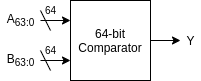
\includegraphics[scale=1]{64bit.png} 
\end{figure}
\pagebreak
\item La tabla describe el comportamiento para distintos bits.

\begin{table}[h!]
\centering
\begin{tabular}{|l|l|l|l|}
\hline
Comparator width &2-input XNOR gates &2-input AND gates&Logic Depth\\
\hline
8 bits&8&7&4\\
\hline
16 bits&16&15&5\\
\hline
32 bits&32&31&6\\
\hline
64 bits&64&63&7\\
\hline
\end{tabular}
\end{table}

\item Se puede proponer que $N = 2^i \ , i\in \{0,1,2,3,4,...\}$, entonces la tabla previa se generaliza a:
\begin{table}[h!]
\centering
\begin{tabular}{|l|l|l|l|}
\hline
Comparator width &2-input XNOR gates &2-input AND gates&Logic Depth\\
\hline
N bits&N&N - 1& i + 1\\
\hline
\end{tabular}
\end{table}
\end{enumerate}

\item El SR-Latch es un circuito secuencial simple que almacena 1 bit. Trabaja con dos inputs S y R, y con  dos outputs $Q $ \ y $\overline{Q}$. Se pueden presentar 4 casos:
\begin{itemize}
\item $S = 1, R = 1:$ este es el caso ``ideal" o ``callado", ya que el valor de $Q$ será el mismo que el de $Q_{prev}$.
\item $S = 0, R = 1:$ este es el caso ``reset", ya que el valor de $Q$ será ``bajado" a 0.
\item $S = 1, R = 0:$ este es el caso ``set", ya que el valor de $Q$ será ``subido" a 1.
\item $S = 0, R = 0:$ este es el caso ``prohibido" o ``metaestable", ya que el valor de $Q$ será el mismo que el de $\overline{Q}$ y los valores asignados a cada uno dependen de las propiedades eléctricas de los transistores que componen las compuertas, mas no de la lógica.

\begin{figure}[h!]
\centering
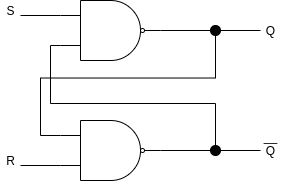
\includegraphics[scale=0.6]{8.png} 
\end{figure}
\pagebreak
\begin{figure}[h!]
\centering
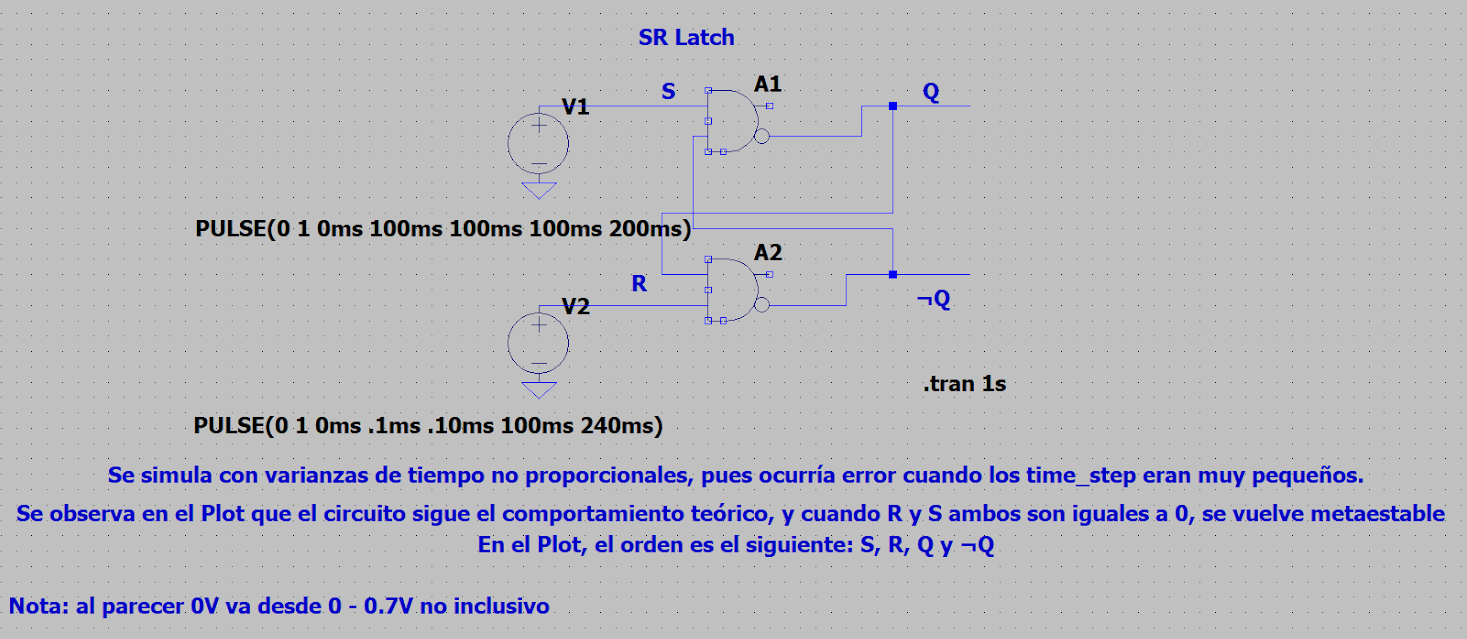
\includegraphics[scale=0.2]{dia5.png} 
\end{figure}
\begin{figure}[h!]
\centering
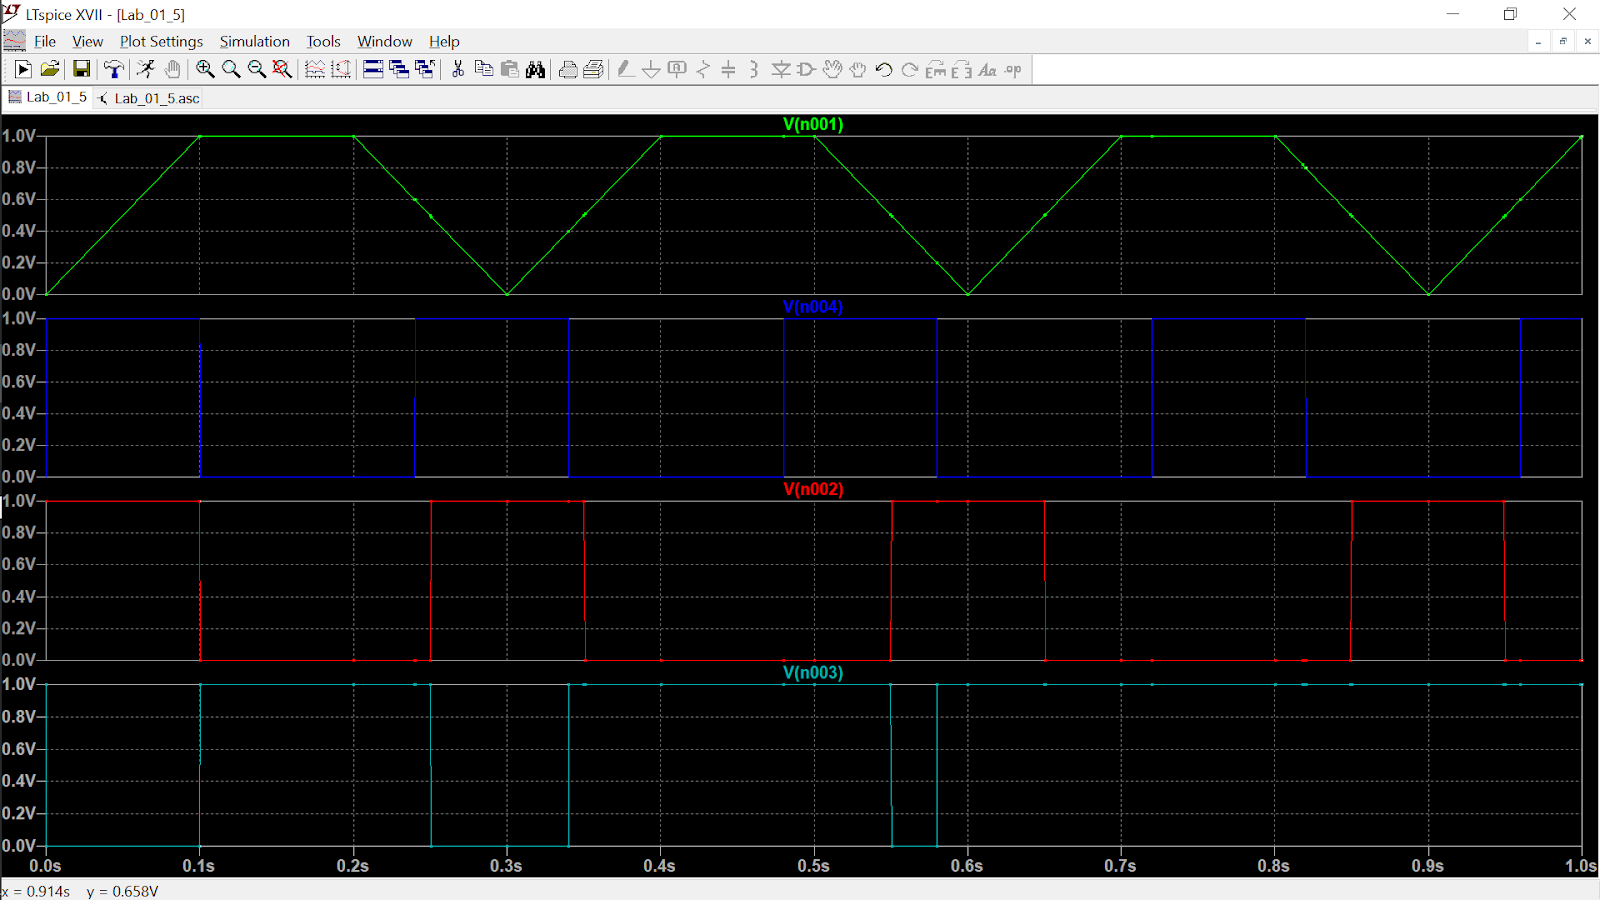
\includegraphics[scale=0.2]{plot5.png} 
\end{figure}

\end{itemize}
\item El Gated D Flip-Flop sirve para regularizar la grabación de datos en los registros, para que la data esté disponible durante todo el ciclo del clock.
Se tienen dos D-Latches, la primera es la maestra y la segunda la esclava. El funcionamiento es simple: cuando el $CLK = 0$, el maestro pasa el valor de $D$ a la ``puerta" del esclavo. Como no se activa su $WE$, entonces el valor de $Q$ será el de $Q_{_{prev}}$.
En el caso contrario, cuando $CLK=1$, el maestro no propaga ningún valor, por lo que el valor de $Q$ será el que ``esperaba en la puerta" del esclavo.
Así, en el ``rising edge" de $0->1$, $Q=D$. En cualquier otro momento $Q$ no varía.
\begin{figure}[h]
\centering
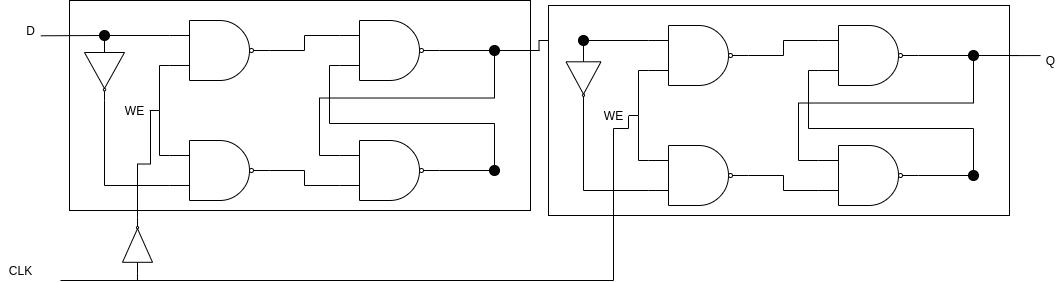
\includegraphics[scale=0.35]{9.png} 
\end{figure}
\begin{figure}[h]
\centering
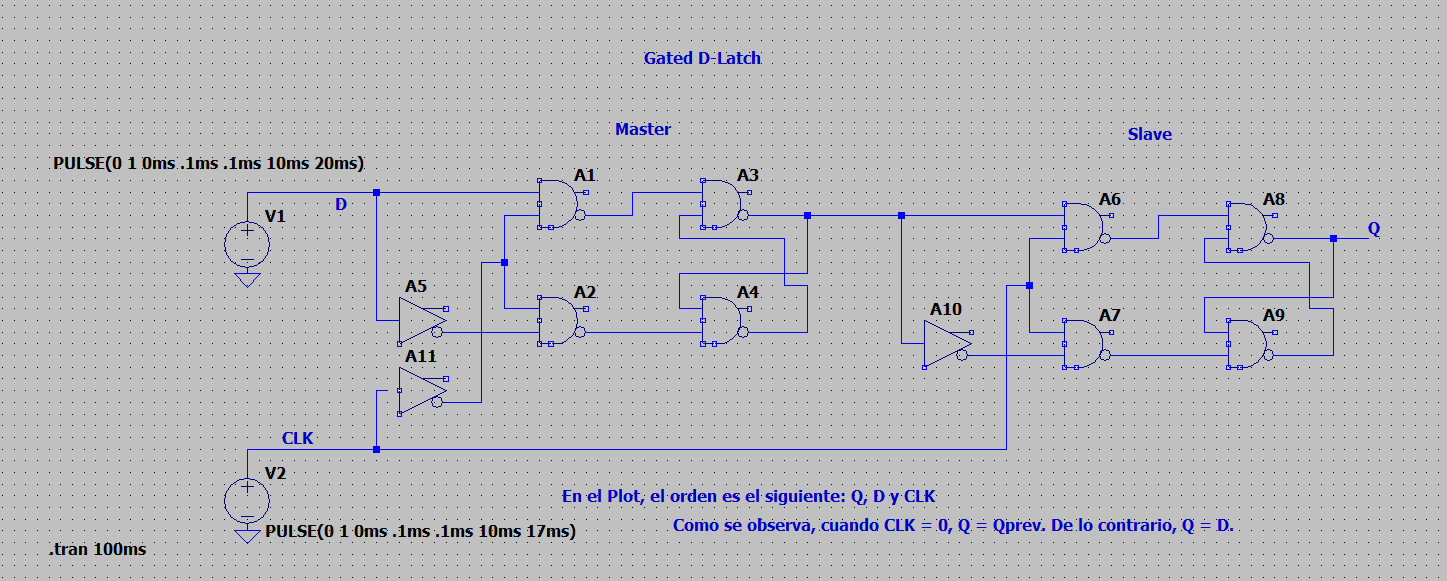
\includegraphics[scale=0.25]{dia6.png} 
\end{figure}
\begin{figure}[h]
\centering
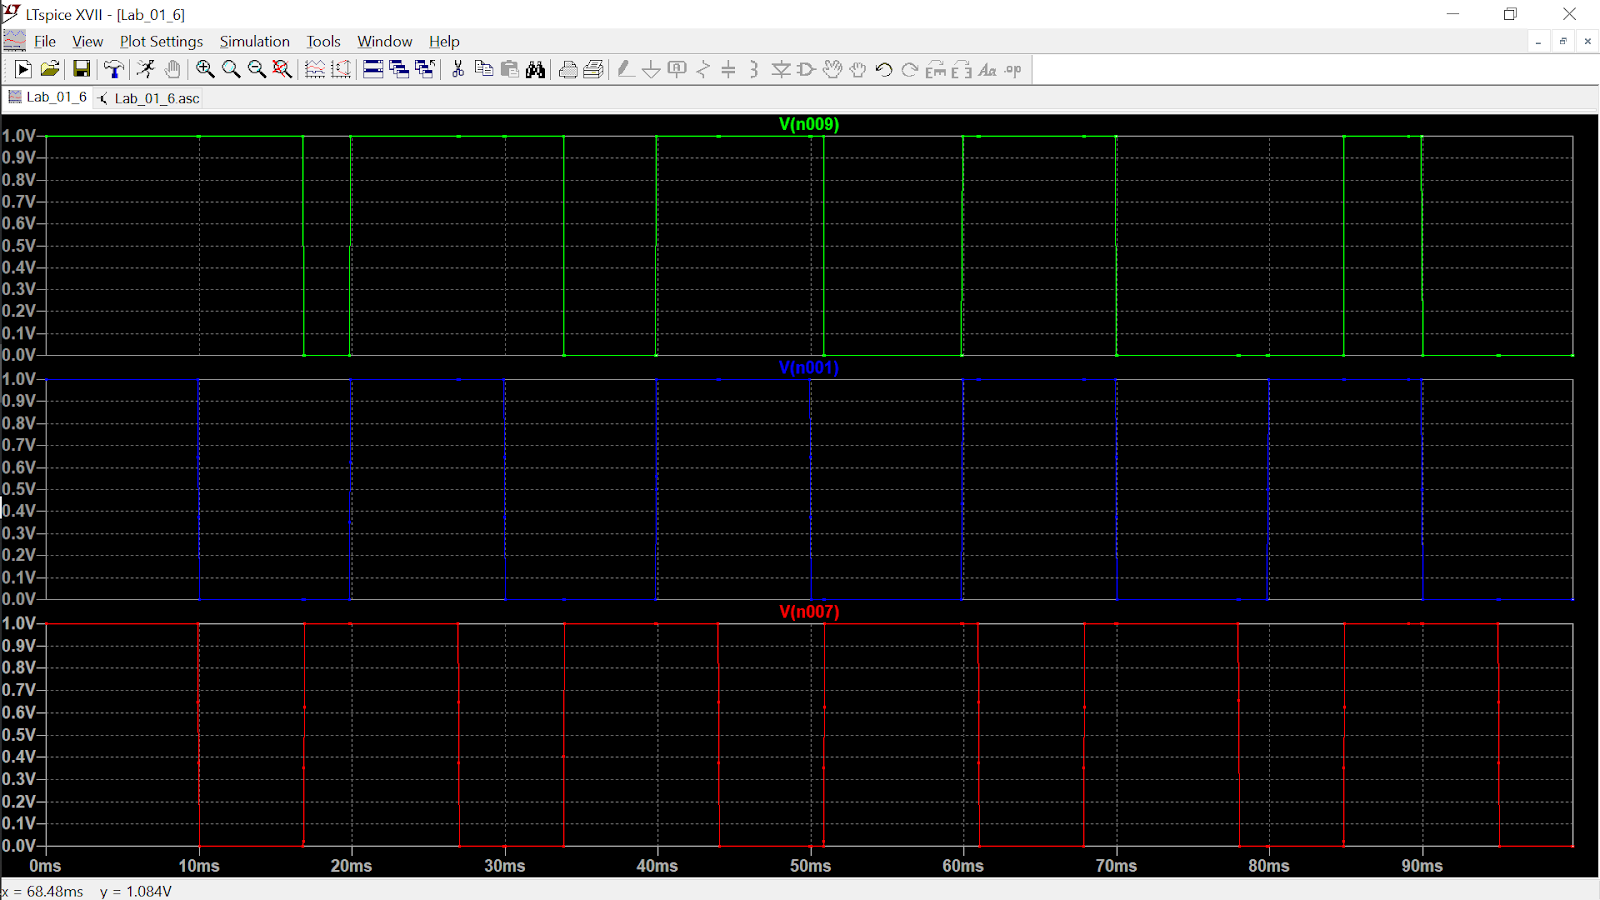
\includegraphics[scale=0.2]{plot6.png} 
\end{figure}
\end{enumerate}


\end{document}